\chapter{VBOs}
Uma das melhorias desta fase em relação à primeira foi a introdução de VBOs no projeto. Com isto a criação das variadas figuras geométricas torna-se mais eficiente.

As definições que foram apresentadas anteriormente para as primitivas são do tipo imediato isto é para cada ponto é usada a função do \textit{OpenGL glVertex3f()}. Contudo o \textit{OpenGL} permite a utilização de \textit{buffers} de arrays. Nestes podemos organizar os atributos dos vértices (coordenadas, coordenadas de texturas e normais). O procedimento a seguir com VBOs é o seguinte:

\begin{enumerate}
	\item Ativar buffers (glEnableClientState(GL VERTEX ARRAY);
	\item  Alocar e preencher os arrays;
	\item  Gerar VBOs;
	\item Preparar desenho dos VBOs;
	\item Desenhar com VBOs.
\end{enumerate}

A estrutura de dados da implementação em VBO’s é semelhante à implementada nos modelos, mas existe uma pequena alteração, pois quando estamos nos modelos temos os pontos que vamos usar numa estrutura definida por nós (Ponto3D), em VBO’s temos de seguir o que é pré-definido, sendo que os pontos são passados em arrays de valores. \\
\\
De seguida pode ser visualizada a estrutura de armazenamento das figuras em VBO's
\begin{verbatim}
struct sVBO {
	char name[256];
	GLuint *buffers;
	unsigned short indices;
	int n_ind;
}
\end{verbatim}


\chapter{Curvas de Catmull-Rom}

A matriz M utilizada para o cálculo da suavidade da curva é a seguinte: \\
\\
float m[4][4] = $\left[ \begin{array}{cccc}
-0.5 & 1.5  & -1.5 & 0.5 \\ 
1.0 & -2.5 & 2 & -0.5\\
-0.5 & 0.0  & 0.5 &0.0\\
0.0 & 1.0 & 0.0 & 0.0
\end{array} \right]$
\\ 
\section{Translações }
As translações à volta de um ponto, que são usadas para os planetas à volta do sol, e os satélites à volta dos planetas têm por base curvas de \textit{Catmull-Rom}. Para tal, são definidos pelo menos quatro pontos de controlo no \textit{xml} e, a cada instante, o objeto é deslocado para a próxima posição nessa curva.

\begin{verbatim}
currentTime = sum(glutGet(GLUT_ELAPSED_TIME))
t=(currentTime%period)/period
\end{verbatim}

Ou seja, calculando a divisão entre o resto do tempo atual com a duração do periodo e a duração do período obté-se um valor entre 0 e 1 que permite calcular ciclicamente qual o próximo ponto onde, dentro da curva, o objeto se deve encontrar.

Para além do tempo, só os pontos de controlo, que permitem gerar a curva, é que são precisos guardar na estrutura de dados.

\chapter{Rotações}

As rotações à volta de um eixo, são usadas para a rotação dos planetas em torno de si mesmos. Para tal, a cada iteração é necessário ajustar o ângulo da rotação.

\begin{verbatim}
currentTime = sum(glutGet(GLUT_ELAPSED_TIME))
angle=((currentTime%period)/period) *360
\end{verbatim}

Ou seja, como anteriormente, calculando a divisão entre o resto do tempo atual com a duração do periodo e a duração do periodo obtém-se um valor entre 0 e 1 que é de seguida multiplicado por 360 para obter o ângulo da rotação.


\chapter{Superfícies de Bezier}

Nesta terceira fase foi proposta a criação de Superfícies de \textit{Bezier}, através de um ficheiro passado como argumento, com as \textit{patches} e os \textit{control points} necessários para a criação da superfície, com o qual o \textit{generator} deve criar a lista de vértices necessários para a criação da superfície. Para ser possível criar as superfícies teve de se fazer algumas alterações no \textit{generator}, assim como novas funções que permitem gerar os vértices pretendidos. 


\section{Ficheiro}
O ficheiro, passado como argumento no \textit{generator}, contém diversas linhas com significados diferentes. A primeira linha contem o número, n, de \textit{patches} necessárias para a criação das superficies, as n linhas seguintes são as linhas das \textit{patches}, cada uma destas aponta para 16 \textit{control points} cada. A seguir aparece uma linha com o número, m, de \textit{control points} presentes no ficheiro, porém, as últimas m linhas são as linhas dos \textit{control points}, cada uma destas linhas contém três valores diferentes.
Se aparecer um ficheiro da seguinte forma: 

\begin{verbatim}

2
0, 1, 2, 3, 4, 5, 6, 7, 8, 9, 10, 11, 12, 13, 14, 15
3, 16, 17, 18, 7, 19, 20, 21, 11, 22, 23, 24, 15, 25, 26, 27
16
1.4, 0, 2.4
1.4, -0.784, 2.4
0.784, -1.4, 2.4
0, -1.4, 2.4
1.3375, 0, 2.53125
1.3375, -0.749, 2.53125
0.749, -1.3375, 2.53125
0, -1.3375, 2.53125
1.4375, 0, 2.53125
1.4375, -0.805, 2.53125
0.805, -1.4375, 2.53125
0, -1.4375, 2.53125
1.5, 0, 2.4
1.5, -0.84, 2.4
0.84, -1.5, 2.4
0, -1.5, 2.4
\end{verbatim}

Sabemos que há duas patches: 

\begin{verbatim}
0, 1, 2, 3, 4, 5, 6, 7, 8, 9, 10, 11, 12, 13, 14, 15
\end{verbatim}

e \begin{verbatim}
3, 16, 17, 18, 7, 19, 20, 21, 11, 22, 23, 24, 15, 25, 26, 27
\end{verbatim}

Haverá também dezasseis \textit{control points} onde 1.4, 0, 2.4 corresponde ao \textit{control point} de índice 0 e  1.4, -0.784, 2.4 \textit{control point} de índice 1 e assim sucessivamente.


\section{Criação da Superfície}


Para o cálculo dos vértices é usada a seguinte fórmula:
\begin{figure}[htpb]
	\centering
	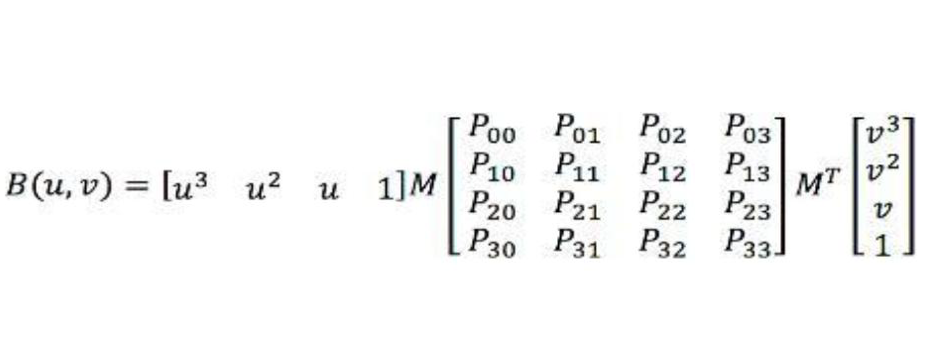
\includegraphics[scale=0.6]{imagens/bezier.png}
	\caption{Fórmula da superfície de Bezier}
	\label{p1:fig:p1_bezier}
\end{figure}

Portanto utilizou-se a seguinte matriz M: \\
float m[4][4] = $\left[ \begin{array}{cccc}
	-1 & 3  & -3 & 1 \\ 
	3 & -6 & 3 & 0\\
	-3 & 3  & 0 &0\\
	1 & 0 & 0 & 0
	\end{array} \right]$
	\\

Para cada vértice precisamos de um valor em x, outro em y e por fim em z. Para tal ser possivel, vamos ter que calcular B(u,v) três vezes, uma com a matriz de todos os x de uma dada \textit{patch}, outra com a matriz de pontos de todos os y e a última para a matriz de pontos de todos os z.


\chapter{Demo}

Neste fase atualizou-se o demo para, ao invés de uma estrutura estática, apresentar movimento. A principal alteração foi animar os objetos. Para tal, introduziu-se extensões aos elementos \textit{translate} e \textit{rotate}, um atributo tempo descreve a duraçãoo para cada rotação ou translação em 360º. 



Assim um planeta pode estar afeto por uma rotação (inclinação), uma velocidade de rotação (rotação em torno de um eixo próprio), uma translação (em redor a um ponto) e uma deslocação (translação). Isto com o minímo
de dois grupos, visto que cada grupo só pode conter uma translação e uma rotação. 